% Options for packages loaded elsewhere
\PassOptionsToPackage{unicode}{hyperref}
\PassOptionsToPackage{hyphens}{url}
%
\documentclass[
  9pt,
  ignorenonframetext,
  aspectratio=169]{beamer}
\usepackage{pgfpages}
\setbeamertemplate{caption}[numbered]
\setbeamertemplate{caption label separator}{: }
\setbeamercolor{caption name}{fg=normal text.fg}
\beamertemplatenavigationsymbolsempty
% Prevent slide breaks in the middle of a paragraph
\widowpenalties 1 10000
\raggedbottom
\setbeamertemplate{part page}{
  \centering
  \begin{beamercolorbox}[sep=16pt,center]{part title}
    \usebeamerfont{part title}\insertpart\par
  \end{beamercolorbox}
}
\setbeamertemplate{section page}{
  \centering
  \begin{beamercolorbox}[sep=12pt,center]{part title}
    \usebeamerfont{section title}\insertsection\par
  \end{beamercolorbox}
}
\setbeamertemplate{subsection page}{
  \centering
  \begin{beamercolorbox}[sep=8pt,center]{part title}
    \usebeamerfont{subsection title}\insertsubsection\par
  \end{beamercolorbox}
}
\AtBeginPart{
  \frame{\partpage}
}
\AtBeginSection{
  \ifbibliography
  \else
    \frame{\sectionpage}
  \fi
}
\AtBeginSubsection{
  \frame{\subsectionpage}
}
\usepackage{lmodern}
\usepackage{amssymb,amsmath}
\usepackage{ifxetex,ifluatex}
\ifnum 0\ifxetex 1\fi\ifluatex 1\fi=0 % if pdftex
  \usepackage[T1]{fontenc}
  \usepackage[utf8]{inputenc}
  \usepackage{textcomp} % provide euro and other symbols
\else % if luatex or xetex
  \usepackage{unicode-math}
  \defaultfontfeatures{Scale=MatchLowercase}
  \defaultfontfeatures[\rmfamily]{Ligatures=TeX,Scale=1}
\fi
\usetheme[]{Berkeley}
\usecolortheme{dove}
\usefonttheme{structurebold}
% Use upquote if available, for straight quotes in verbatim environments
\IfFileExists{upquote.sty}{\usepackage{upquote}}{}
\IfFileExists{microtype.sty}{% use microtype if available
  \usepackage[]{microtype}
  \UseMicrotypeSet[protrusion]{basicmath} % disable protrusion for tt fonts
}{}
\makeatletter
\@ifundefined{KOMAClassName}{% if non-KOMA class
  \IfFileExists{parskip.sty}{%
    \usepackage{parskip}
  }{% else
    \setlength{\parindent}{0pt}
    \setlength{\parskip}{6pt plus 2pt minus 1pt}}
}{% if KOMA class
  \KOMAoptions{parskip=half}}
\makeatother
\usepackage{xcolor}
\IfFileExists{xurl.sty}{\usepackage{xurl}}{} % add URL line breaks if available
\IfFileExists{bookmark.sty}{\usepackage{bookmark}}{\usepackage{hyperref}}
\hypersetup{
  pdftitle={Regressão Linear},
  pdfauthor={Frederico Bertholini},
  hidelinks,
  pdfcreator={LaTeX via pandoc}}
\urlstyle{same} % disable monospaced font for URLs
\newif\ifbibliography
\usepackage{color}
\usepackage{fancyvrb}
\newcommand{\VerbBar}{|}
\newcommand{\VERB}{\Verb[commandchars=\\\{\}]}
\DefineVerbatimEnvironment{Highlighting}{Verbatim}{commandchars=\\\{\}}
% Add ',fontsize=\small' for more characters per line
\usepackage{framed}
\definecolor{shadecolor}{RGB}{248,248,248}
\newenvironment{Shaded}{\begin{snugshade}}{\end{snugshade}}
\newcommand{\AlertTok}[1]{\textcolor[rgb]{0.94,0.16,0.16}{#1}}
\newcommand{\AnnotationTok}[1]{\textcolor[rgb]{0.56,0.35,0.01}{\textbf{\textit{#1}}}}
\newcommand{\AttributeTok}[1]{\textcolor[rgb]{0.77,0.63,0.00}{#1}}
\newcommand{\BaseNTok}[1]{\textcolor[rgb]{0.00,0.00,0.81}{#1}}
\newcommand{\BuiltInTok}[1]{#1}
\newcommand{\CharTok}[1]{\textcolor[rgb]{0.31,0.60,0.02}{#1}}
\newcommand{\CommentTok}[1]{\textcolor[rgb]{0.56,0.35,0.01}{\textit{#1}}}
\newcommand{\CommentVarTok}[1]{\textcolor[rgb]{0.56,0.35,0.01}{\textbf{\textit{#1}}}}
\newcommand{\ConstantTok}[1]{\textcolor[rgb]{0.00,0.00,0.00}{#1}}
\newcommand{\ControlFlowTok}[1]{\textcolor[rgb]{0.13,0.29,0.53}{\textbf{#1}}}
\newcommand{\DataTypeTok}[1]{\textcolor[rgb]{0.13,0.29,0.53}{#1}}
\newcommand{\DecValTok}[1]{\textcolor[rgb]{0.00,0.00,0.81}{#1}}
\newcommand{\DocumentationTok}[1]{\textcolor[rgb]{0.56,0.35,0.01}{\textbf{\textit{#1}}}}
\newcommand{\ErrorTok}[1]{\textcolor[rgb]{0.64,0.00,0.00}{\textbf{#1}}}
\newcommand{\ExtensionTok}[1]{#1}
\newcommand{\FloatTok}[1]{\textcolor[rgb]{0.00,0.00,0.81}{#1}}
\newcommand{\FunctionTok}[1]{\textcolor[rgb]{0.00,0.00,0.00}{#1}}
\newcommand{\ImportTok}[1]{#1}
\newcommand{\InformationTok}[1]{\textcolor[rgb]{0.56,0.35,0.01}{\textbf{\textit{#1}}}}
\newcommand{\KeywordTok}[1]{\textcolor[rgb]{0.13,0.29,0.53}{\textbf{#1}}}
\newcommand{\NormalTok}[1]{#1}
\newcommand{\OperatorTok}[1]{\textcolor[rgb]{0.81,0.36,0.00}{\textbf{#1}}}
\newcommand{\OtherTok}[1]{\textcolor[rgb]{0.56,0.35,0.01}{#1}}
\newcommand{\PreprocessorTok}[1]{\textcolor[rgb]{0.56,0.35,0.01}{\textit{#1}}}
\newcommand{\RegionMarkerTok}[1]{#1}
\newcommand{\SpecialCharTok}[1]{\textcolor[rgb]{0.00,0.00,0.00}{#1}}
\newcommand{\SpecialStringTok}[1]{\textcolor[rgb]{0.31,0.60,0.02}{#1}}
\newcommand{\StringTok}[1]{\textcolor[rgb]{0.31,0.60,0.02}{#1}}
\newcommand{\VariableTok}[1]{\textcolor[rgb]{0.00,0.00,0.00}{#1}}
\newcommand{\VerbatimStringTok}[1]{\textcolor[rgb]{0.31,0.60,0.02}{#1}}
\newcommand{\WarningTok}[1]{\textcolor[rgb]{0.56,0.35,0.01}{\textbf{\textit{#1}}}}
\usepackage{graphicx}
\makeatletter
\def\maxwidth{\ifdim\Gin@nat@width>\linewidth\linewidth\else\Gin@nat@width\fi}
\def\maxheight{\ifdim\Gin@nat@height>\textheight\textheight\else\Gin@nat@height\fi}
\makeatother
% Scale images if necessary, so that they will not overflow the page
% margins by default, and it is still possible to overwrite the defaults
% using explicit options in \includegraphics[width, height, ...]{}
\setkeys{Gin}{width=\maxwidth,height=\maxheight,keepaspectratio}
% Set default figure placement to htbp
\makeatletter
\def\fps@figure{htbp}
\makeatother
\setlength{\emergencystretch}{3em} % prevent overfull lines
\providecommand{\tightlist}{%
  \setlength{\itemsep}{0pt}\setlength{\parskip}{0pt}}
\setcounter{secnumdepth}{5}

\title{Regressão Linear}
\subtitle{Métodos Quantitativos Aplicados à Ciência Política}
\author{Frederico Bertholini}
\date{14.dez.2020}

\begin{document}
\frame{\titlepage}

\begin{frame}[allowframebreaks]
  \tableofcontents[hideallsubsections]
\end{frame}
\begin{frame}{Conceitos}
\protect\hypertarget{conceitos}{}
Modelos de regressão estabelecem relações entre variáveis.

Isso é feito através de uma equação que expressa uma variável
\textbf{dependente} em termos de uma ou mais variáveis
\textbf{independentes}.
\end{frame}

\begin{frame}[fragile]{Visualizando relações entre variáveis}
\protect\hypertarget{visualizando-relauxe7uxf5es-entre-variuxe1veis}{}
\begin{Shaded}
\begin{Highlighting}[]
\NormalTok{legenda }\OperatorTok{\%\textgreater{}\%}\StringTok{ }\KeywordTok{ggplot}\NormalTok{(}\KeywordTok{aes}\NormalTok{(}\DataTypeTok{x =}\NormalTok{ DOAPFIS, }\DataTypeTok{y =}\NormalTok{ VOTLEG)) }\OperatorTok{+}\StringTok{ }
\StringTok{  }\KeywordTok{geom\_point}\NormalTok{() }\OperatorTok{+}\StringTok{ }\CommentTok{\# Adiciona os pontos}
\StringTok{  }\KeywordTok{geom\_smooth}\NormalTok{(}\DataTypeTok{method =} \StringTok{"lm"}\NormalTok{,}\DataTypeTok{se=}\NormalTok{F) }\OperatorTok{+}\StringTok{ }\CommentTok{\# Adiciona a curva, estimada por um modelo linear}
\StringTok{  }\KeywordTok{labs}\NormalTok{(}\DataTypeTok{x=}\StringTok{""}\NormalTok{,}\DataTypeTok{y=}\StringTok{""}\NormalTok{)}
\end{Highlighting}
\end{Shaded}

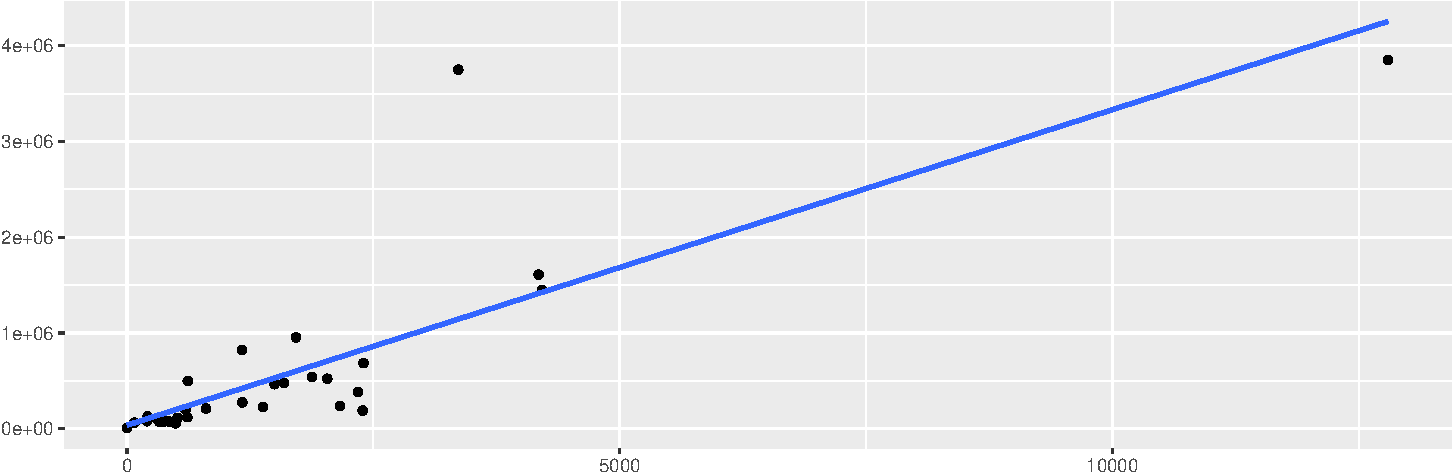
\includegraphics{aula_12_files/figure-beamer/unnamed-chunk-1-1.pdf}
\end{frame}

\begin{frame}{}
\protect\hypertarget{section}{}
Tendência geral: \(VOTLEG = \beta_0 + \beta_1 DOAPFIS\)

4 perguntas importantes:

Quem é a varável dependente?

Quem é a independente?

Qual é o significado de \(\beta_1\)?

Qual é o significado de \(\beta_0\)?
\end{frame}

\begin{frame}{\(\beta_0\)}
\protect\hypertarget{beta_0}{}
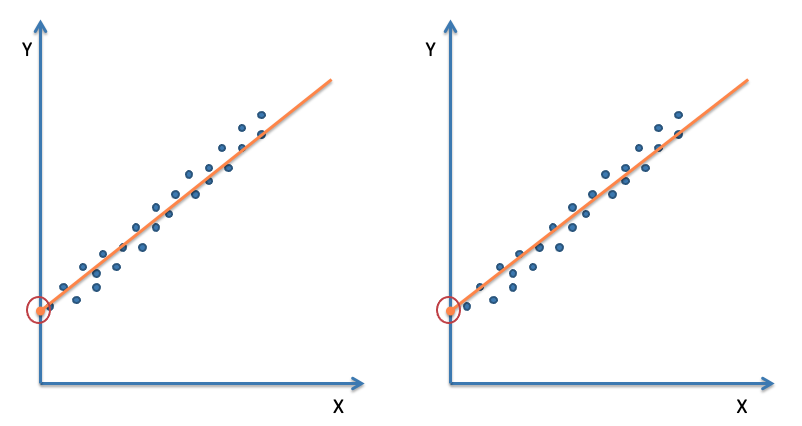
\includegraphics{imgs/beta0.png}
\end{frame}

\begin{frame}{\(\beta_1\)}
\protect\hypertarget{beta_1}{}
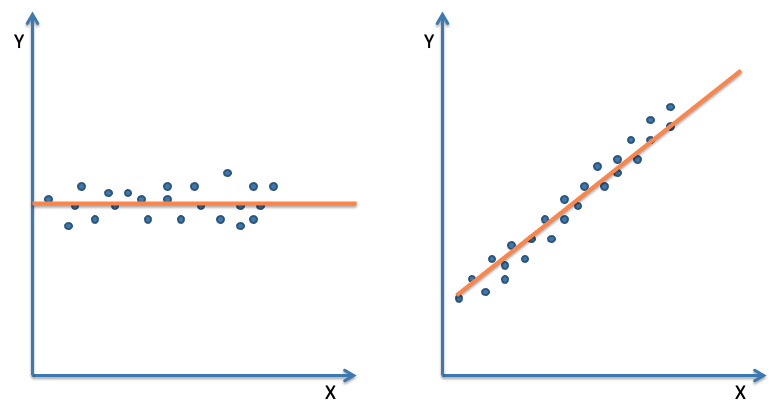
\includegraphics{imgs/beta1.png}
\end{frame}

\begin{frame}{}
\protect\hypertarget{section-1}{}
X e Y estão relacionadas. Esta relação ocorre para todos os X´s e Y´s.

Nós coletamos alguns dados e possuímos apenas uma amostra de toda a
população de X e Y. Observando a relação entre os X's e Y's da nossa
amostra, nós tentamos estimar a relação entre X e Y na população.

\[
Y_i = \beta_0 + \beta_1 x_{i1} + \epsilon_i
\]

\[
Y_{i}=\hat{\beta}_{0}+\hat{\beta}_{1} X_{i}+\hat{\varepsilon}_{i}
\]

\[
\hat{Y}=b_{0}+b_{1} X
\]
\end{frame}

\begin{frame}{O que estamos testando? (e se \(\beta_1=0\))}
\protect\hypertarget{o-que-estamos-testando-e-se-beta_10}{}
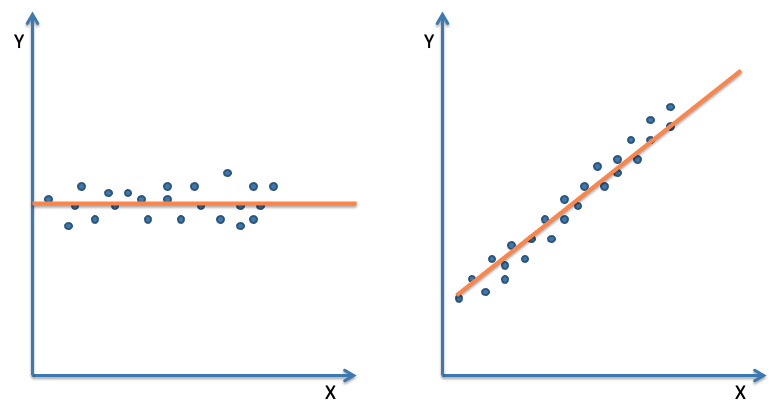
\includegraphics{imgs/beta1.png}
\end{frame}

\begin{frame}{Significância e valor-p da regressão}
\protect\hypertarget{significuxe2ncia-e-valor-p-da-regressuxe3o}{}
\[
\left\{\begin{array}{l}
H_{0}: \beta_{1}=0 \\
H_{A}: \beta_{1} \neq 0
\end{array}\right.
\]

Teste da significância de \(\beta_{1}\):

Valor-p \textless{} o que considerarmos adequado (0,05?) : Rejeita
\(H_{0}\)

-\textgreater{} A relação entre X e Y é \textbf{significante}, ou seja,
tem significância do ponto de vista estatístico.

ps.: Significante é o mesmo que significativo?
\end{frame}

\begin{frame}[fragile]{Estimativas}
\protect\hypertarget{estimativas}{}
\begin{Shaded}
\begin{Highlighting}[]
\NormalTok{(meu\_modelo \textless{}{-}}\StringTok{ }\NormalTok{legenda }\OperatorTok{\%\textgreater{}\%}\StringTok{ }\KeywordTok{lm}\NormalTok{(VOTLEG }\OperatorTok{\textasciitilde{}}\StringTok{ }\NormalTok{DOAPFIS, }\DataTypeTok{data =}\NormalTok{ .))}
\end{Highlighting}
\end{Shaded}

\begin{verbatim}
Call:
lm(formula = VOTLEG ~ DOAPFIS, data = .)

Coefficients:
(Intercept)      DOAPFIS  
    36142.3        329.5  
\end{verbatim}
\end{frame}

\begin{frame}[fragile]{}
\protect\hypertarget{section-2}{}
\begin{Shaded}
\begin{Highlighting}[]
\KeywordTok{get\_regression\_points}\NormalTok{(meu\_modelo) }\OperatorTok{\%\textgreater{}\%}
\StringTok{  }\KeywordTok{ggplot}\NormalTok{(}\KeywordTok{aes}\NormalTok{(}\DataTypeTok{x =}\NormalTok{ residual)) }\OperatorTok{+}
\StringTok{  }\KeywordTok{geom\_histogram}\NormalTok{(}\DataTypeTok{color =} \StringTok{"white"}\NormalTok{) }\OperatorTok{+}
\StringTok{  }\KeywordTok{labs}\NormalTok{(}\DataTypeTok{x =} \StringTok{"Residuos"}\NormalTok{)}
\end{Highlighting}
\end{Shaded}

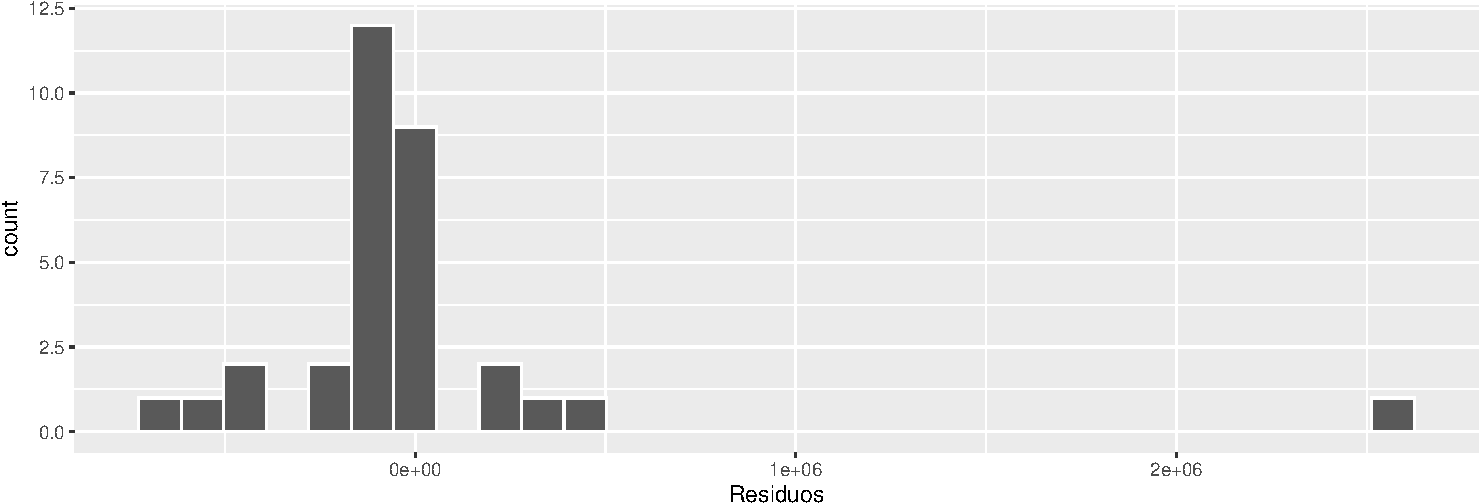
\includegraphics{aula_12_files/figure-beamer/unnamed-chunk-3-1.pdf}
\end{frame}

\begin{frame}[fragile]{Resíduos com \texttt{sjPlot}}
\protect\hypertarget{resuxedduos-com-sjplot}{}
\begin{Shaded}
\begin{Highlighting}[]
\NormalTok{sjPlot}\OperatorTok{::}\KeywordTok{plot\_residuals}\NormalTok{(meu\_modelo)}
\end{Highlighting}
\end{Shaded}

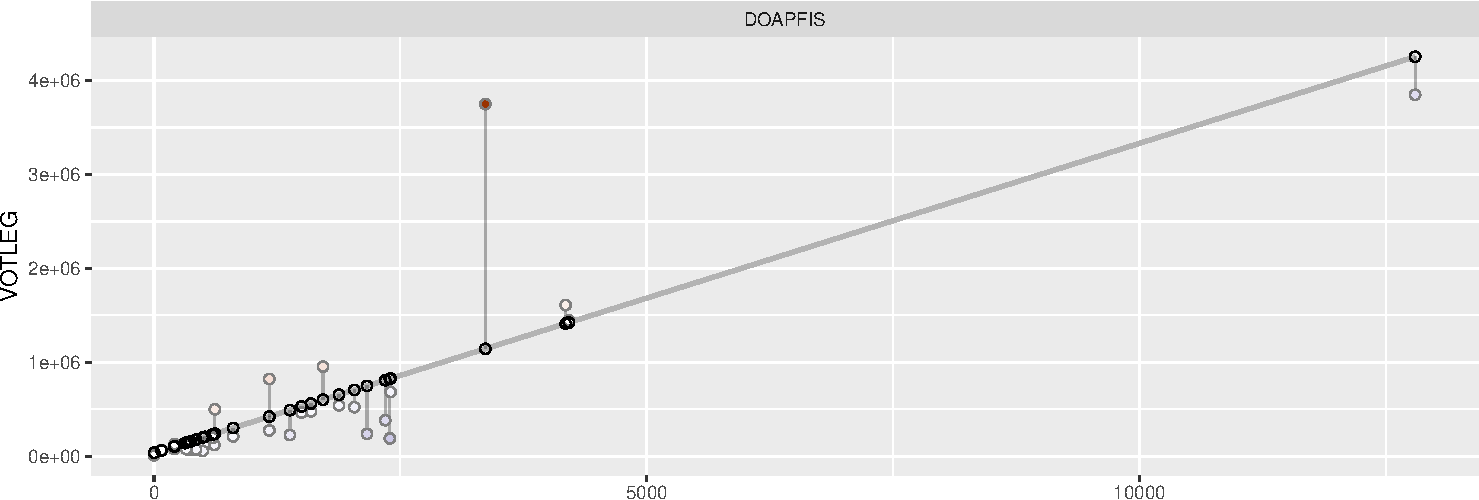
\includegraphics{aula_12_files/figure-beamer/unnamed-chunk-4-1.pdf}
\end{frame}

\begin{frame}{Quais são as características ideais da nossa reta?}
\protect\hypertarget{quais-suxe3o-as-caracteruxedsticas-ideais-da-nossa-reta}{}
Resíduo esperado é zero: \(E(e)=0\)

Erra igualmente para ambos os lados

Erra o mínimo possível
\end{frame}

\begin{frame}{Método dos mínimos quadrados}
\protect\hypertarget{muxe9todo-dos-muxednimos-quadrados}{}
Escolhe uma reta de forma que a soma dos erros ao quadrado seja a menor
possível.

Encontrar os valores de \(b_0\) e \(b_1\) para o qual é o menor
possível.

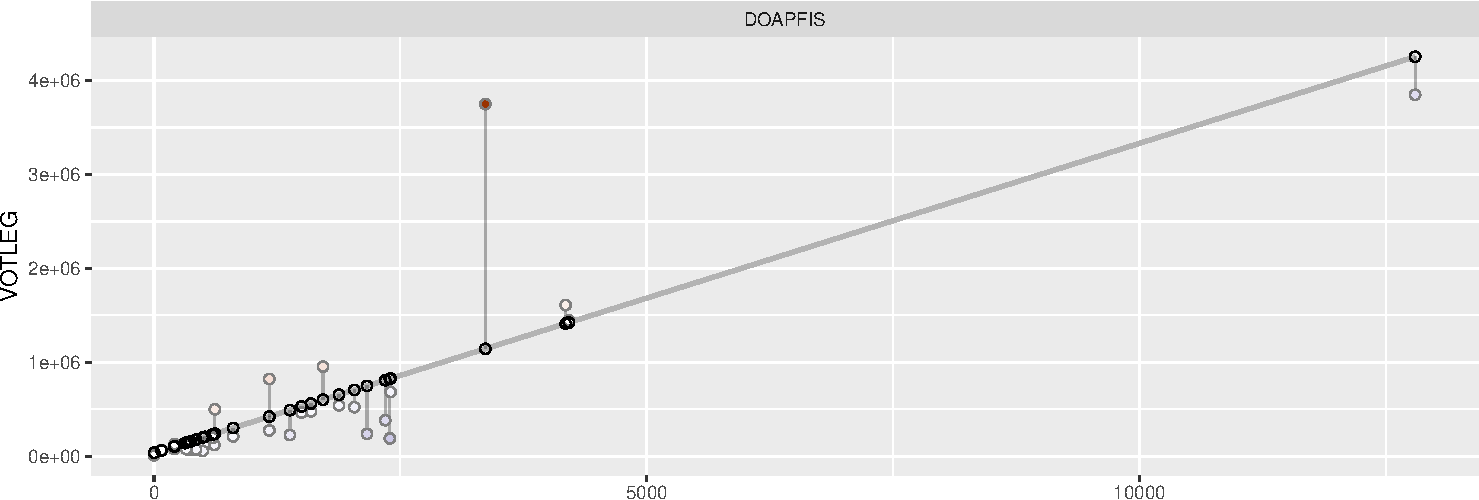
\includegraphics{aula_12_files/figure-beamer/unnamed-chunk-5-1.pdf}
\end{frame}

\begin{frame}{MMQ ou OLS \ldots{}}
\protect\hypertarget{mmq-ou-ols}{}
Encontrar os valores de \(b_0\) e \(b_1\) que minimizem \[
S=\sum_{i}\left[Y_{i}-\left(b_{0}+b_{1} X\right)\right]^{2}
\] Obtemos isso calculando \(b_0\) e \(b_1\) tais que \[
\frac{\partial S}{\partial b_{0}}=0 \quad \frac{\partial S}{\partial b_{1}}=0
\] Resolvendo, chega-se a: \[
b_{1}=\frac{n \sum_{i} X_{i} Y_{i}-\left(\sum_{i} X_{i}\right)\left(\sum_{i} Y_{i}\right)}{n \sum_{i} X_{i}^{2}-\left(\sum_{i} X_{i}\right)^{2}}
\]

\[
b_{0}=\frac{\left(\sum_{i} Y_{i}\right)\left(\sum_{i} X_{i}^{2}\right)-\left(\sum_{i} X_{i}\right)\left(\sum_{i} X_{i} Y_{i}\right)}{n \sum_{i} X_{i}^{2}-\left(\sum_{i} X_{i}\right)^{2}}
\]
\end{frame}

\begin{frame}{\ldots continua}
\protect\hypertarget{continua}{}
Que pode ser escrito como \[
b_{1}=\frac{\operatorname{cov}(X, Y)}{\operatorname{var}(X)}
\]

\[
\bar{Y}=b_{0}+b_{1} \bar{X}
\]
\end{frame}

\begin{frame}{Sob certas premissas, é possível provar que}
\protect\hypertarget{sob-certas-premissas-uxe9-possuxedvel-provar-que}{}
\[
\frac{b_{1}}{s_{b_{1}}} \sim t_{n-2}
\] Onde \[
s_{b_{1}}^{2}=\frac{s^{2}}{\sum_{i}\left(X_{i}-\bar{X}\right)^{2}} \quad s_{e}^{2}=\frac{\sum_{i} e_{i}^{2}}{n-2}
\]

Isto permite:

-- realizar teste de hipóteses com b1, como, por exemplo, testar sua
significância

-- Construir intervalos de confiança e de predição para Y em um valor de
X qualquer
\end{frame}

\begin{frame}{Premissas}
\protect\hypertarget{premissas}{}
Os resíduos devem ser normais, homoscedásticos e independentes.
\end{frame}

\begin{frame}{Normalidade}
\protect\hypertarget{normalidade}{}
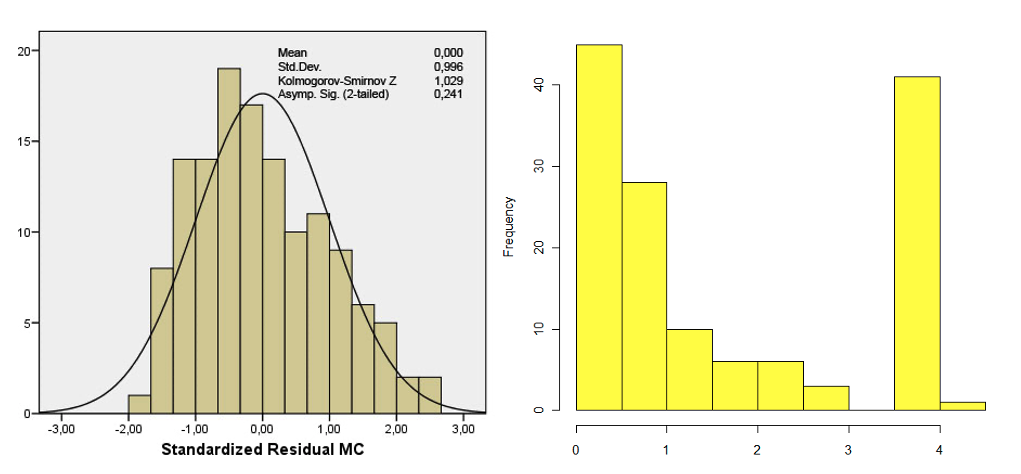
\includegraphics{imgs/norm1.png}
\end{frame}

\begin{frame}{Normalidade}
\protect\hypertarget{normalidade-1}{}
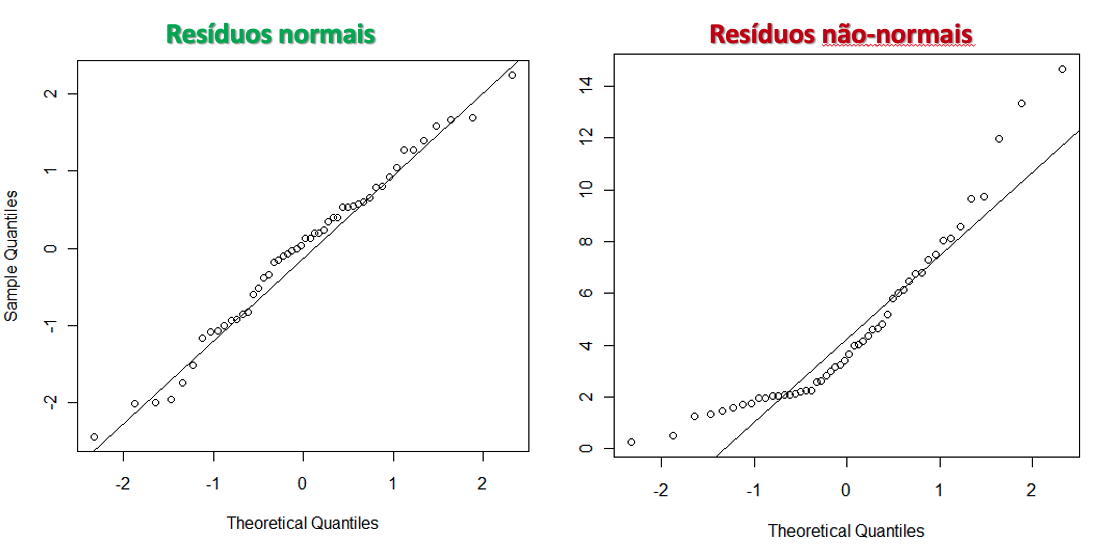
\includegraphics{imgs/norm2.png}
\end{frame}

\begin{frame}{Homocedasticidade}
\protect\hypertarget{homocedasticidade}{}
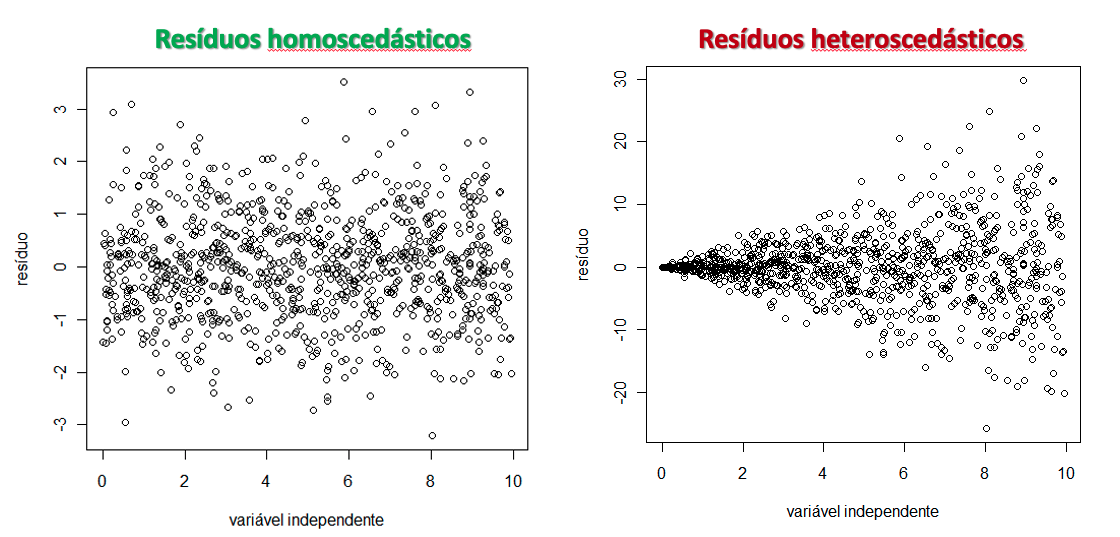
\includegraphics{imgs/homoc.png}
\end{frame}

\begin{frame}{Independência}
\protect\hypertarget{independuxeancia}{}
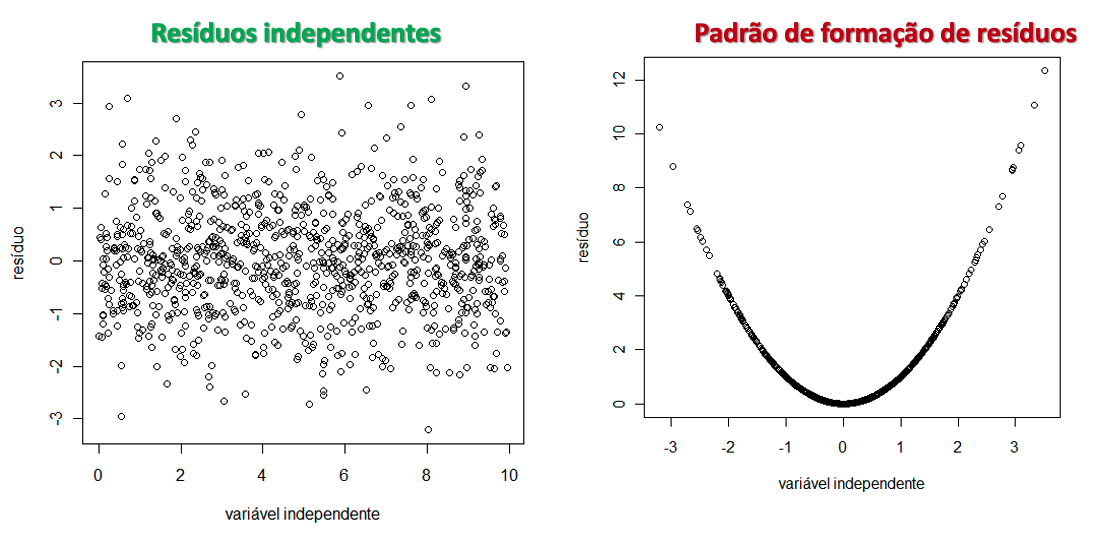
\includegraphics{imgs/indep.png}
\end{frame}

\begin{frame}{\(R^2\)}
\protect\hypertarget{r2}{}
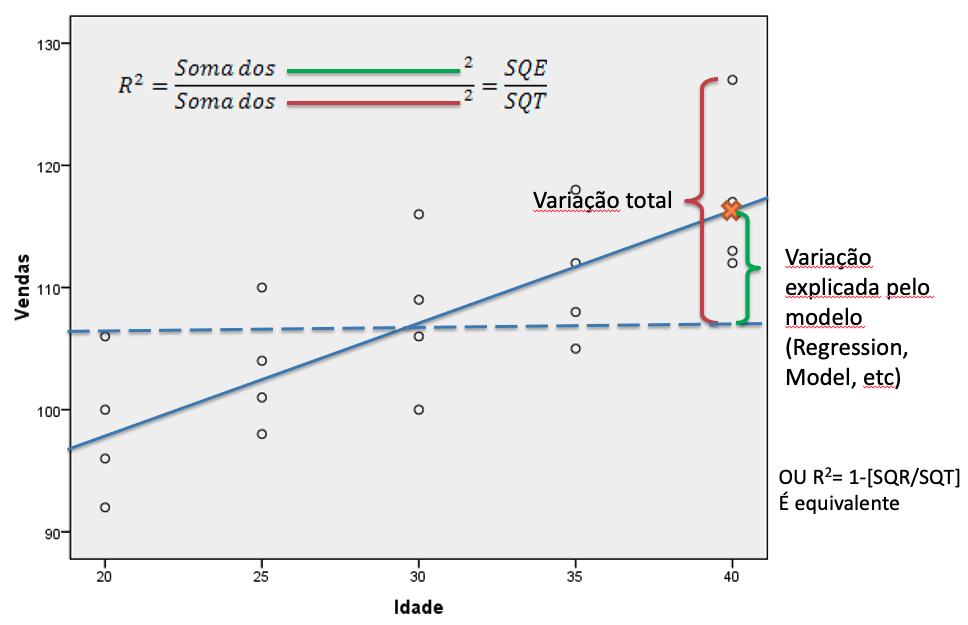
\includegraphics{imgs/r2_explica.png}
\end{frame}

\begin{frame}{Modelos explicativos e preditivos}
\protect\hypertarget{modelos-explicativos-e-preditivos}{}
Modelos de regressão podem servir para explicar ou para prever.

\begin{itemize}
\item
  Em modelos explicativos, o que importa é ter fortes razões para crer
  que as variáveis explicativas influenciam a variável explicada. Isso é
  medido por um valor-p baixo.
\item
  Em modelos preditivos, o que importa é ter um bom ajuste da reta aos
  dados. Isso é medido por um \(R^2\) alto.
\end{itemize}

Modelo preditivo: Previsão eleitoral (electoral forecasting)

Modelo explicativo: total de votos de legenda para deputado federal
(VOTLEG) \textbf{explicado por} número de doações de pessoas físicas
(DOAPFIS)
\end{frame}

\begin{frame}[fragile]{Eliminando outliers}
\protect\hypertarget{eliminando-outliers}{}
\begin{Shaded}
\begin{Highlighting}[]
\NormalTok{legenda }\OperatorTok{\%\textless{}\textgreater{}\%}\StringTok{ }\NormalTok{dplyr}\OperatorTok{::}\KeywordTok{filter}\NormalTok{(DOAPFIS}\OperatorTok{\textless{}}\DecValTok{5000}\NormalTok{,VOTLEG}\OperatorTok{\textless{}}\DecValTok{2000000}\NormalTok{)}
\NormalTok{(meu\_modelo \textless{}{-}}\StringTok{ }\NormalTok{legenda }\OperatorTok{\%\textgreater{}\%}\StringTok{ }\KeywordTok{lm}\NormalTok{(VOTLEG }\OperatorTok{\textasciitilde{}}\StringTok{ }\NormalTok{DOAPFIS, }\DataTypeTok{data =}\NormalTok{ .))}
\end{Highlighting}
\end{Shaded}

\begin{verbatim}
Call:
lm(formula = VOTLEG ~ DOAPFIS, data = .)

Coefficients:
(Intercept)      DOAPFIS  
    -6439.4        304.1  
\end{verbatim}
\end{frame}

\begin{frame}[fragile]{Usando \texttt{tidy}}
\protect\hypertarget{usando-tidy}{}
\begin{Shaded}
\begin{Highlighting}[]
\KeywordTok{tidy}\NormalTok{(meu\_modelo)}
\end{Highlighting}
\end{Shaded}

\begin{verbatim}
# A tibble: 2 x 5
  term        estimate std.error statistic       p.value
  <chr>          <dbl>     <dbl>     <dbl>         <dbl>
1 (Intercept)   -6439.   58572.     -0.110 0.913        
2 DOAPFIS         304.      35.9     8.47  0.00000000325
\end{verbatim}
\end{frame}

\begin{frame}[fragile]{Usando \texttt{glance}}
\protect\hypertarget{usando-glance}{}
\begin{Shaded}
\begin{Highlighting}[]
\KeywordTok{glance}\NormalTok{(meu\_modelo)}
\end{Highlighting}
\end{Shaded}

\begin{verbatim}
# A tibble: 1 x 12
  r.squared adj.r.squared  sigma statistic p.value    df logLik   AIC   BIC
      <dbl>         <dbl>  <dbl>     <dbl>   <dbl> <dbl>  <dbl> <dbl> <dbl>
1     0.719         0.709 2.16e5      71.8 3.25e-9     1  -410.  826.  830.
# ... with 3 more variables: deviance <dbl>, df.residual <int>, nobs <int>
\end{verbatim}
\end{frame}

\begin{frame}[fragile]{Resíduos com \texttt{sjPlot}}
\protect\hypertarget{resuxedduos-com-sjplot-1}{}
\begin{Shaded}
\begin{Highlighting}[]
\NormalTok{sjPlot}\OperatorTok{::}\KeywordTok{plot\_residuals}\NormalTok{(meu\_modelo)}
\end{Highlighting}
\end{Shaded}

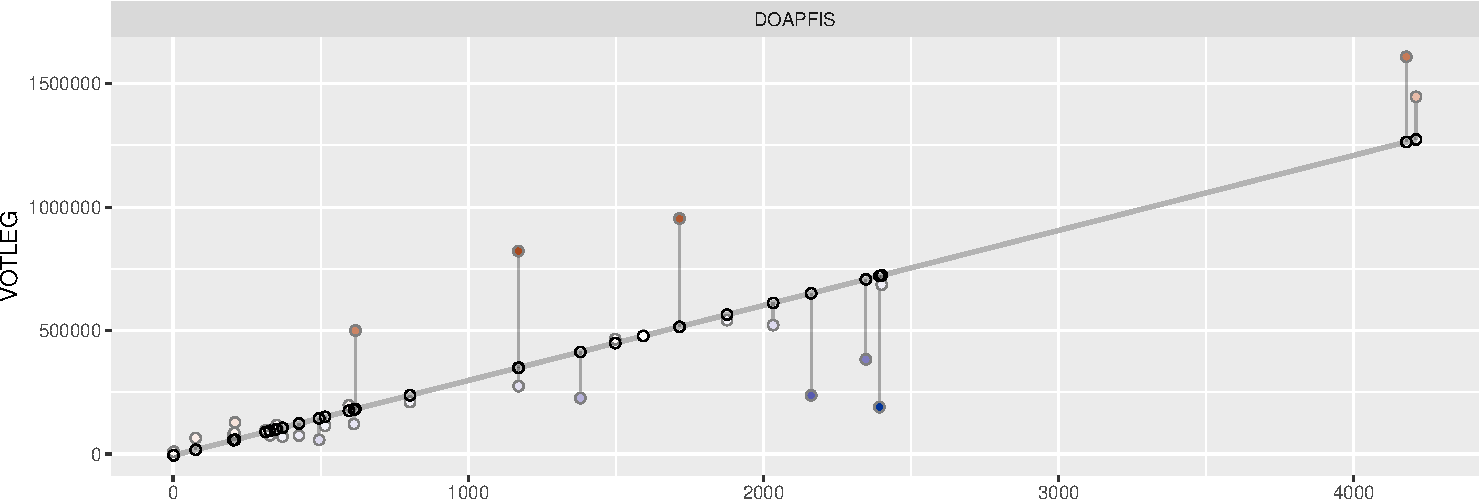
\includegraphics{aula_12_files/figure-beamer/unnamed-chunk-9-1.pdf}
\end{frame}

\begin{frame}[fragile]{Inferência}
\protect\hypertarget{inferuxeancia}{}
NC = 95\%

\begin{Shaded}
\begin{Highlighting}[]
\KeywordTok{confint}\NormalTok{(meu\_modelo, }\DataTypeTok{level =} \FloatTok{0.95}\NormalTok{)}
\end{Highlighting}
\end{Shaded}

\begin{verbatim}
                  2.5 %      97.5 %
(Intercept) -126418.782 113539.9612
DOAPFIS         230.576    377.5736
\end{verbatim}

NC = 90\%

\begin{Shaded}
\begin{Highlighting}[]
\KeywordTok{confint}\NormalTok{(meu\_modelo, }\DataTypeTok{level =} \FloatTok{0.90}\NormalTok{)}
\end{Highlighting}
\end{Shaded}

\begin{verbatim}
                     5 %      95 %
(Intercept) -106078.1080 93199.288
DOAPFIS         243.0366   365.113
\end{verbatim}
\end{frame}

\begin{frame}[fragile]{É possível salvar o \emph{output} da função
\texttt{summary}}
\protect\hypertarget{uxe9-possuxedvel-salvar-o-output-da-funuxe7uxe3o-summary}{}
\begin{Shaded}
\begin{Highlighting}[]
\NormalTok{(resumo \textless{}{-}}\StringTok{ }\KeywordTok{summary}\NormalTok{(meu\_modelo))}
\end{Highlighting}
\end{Shaded}

\begin{verbatim}
Call:
lm(formula = VOTLEG ~ DOAPFIS, data = .)

Residuals:
    Min      1Q  Median      3Q     Max 
-531447  -56292   -8653   27238  472375 

Coefficients:
            Estimate Std. Error t value Pr(>|t|)    
(Intercept) -6439.41   58572.03  -0.110    0.913    
DOAPFIS       304.07      35.88   8.475 3.25e-09 ***
---
Signif. codes:  0 '***' 0.001 '**' 0.01 '*' 0.05 '.' 0.1 ' ' 1

Residual standard error: 215600 on 28 degrees of freedom
Multiple R-squared:  0.7195,    Adjusted R-squared:  0.7095 
F-statistic: 71.82 on 1 and 28 DF,  p-value: 3.249e-09
\end{verbatim}
\end{frame}

\begin{frame}[fragile]{Obtendo resultados detalhados}
\protect\hypertarget{obtendo-resultados-detalhados}{}
\begin{Shaded}
\begin{Highlighting}[]
\NormalTok{meu\_modelo}\OperatorTok{$}\NormalTok{coefficients}
\end{Highlighting}
\end{Shaded}

\begin{verbatim}
(Intercept)     DOAPFIS 
 -6439.4103    304.0748 
\end{verbatim}
\end{frame}

\begin{frame}[fragile]{Outras informações salvas dentro do objeto podem
ser vistas com \texttt{names}:}
\protect\hypertarget{outras-informauxe7uxf5es-salvas-dentro-do-objeto-podem-ser-vistas-com-names}{}
\begin{Shaded}
\begin{Highlighting}[]
\KeywordTok{names}\NormalTok{(meu\_modelo)}
\end{Highlighting}
\end{Shaded}

\begin{verbatim}
 [1] "coefficients"  "residuals"     "effects"       "rank"         
 [5] "fitted.values" "assign"        "qr"            "df.residual"  
 [9] "xlevels"       "call"          "terms"         "model"        
\end{verbatim}

\(R^2\)

\begin{Shaded}
\begin{Highlighting}[]
\NormalTok{resumo}\OperatorTok{$}\NormalTok{r.squared}
\end{Highlighting}
\end{Shaded}

\begin{verbatim}
[1] 0.7194894
\end{verbatim}
\end{frame}

\begin{frame}[fragile]{}
\protect\hypertarget{section-3}{}
\begin{Shaded}
\begin{Highlighting}[]
\NormalTok{sjPlot}\OperatorTok{::}\KeywordTok{plot\_model}\NormalTok{(meu\_modelo)}
\end{Highlighting}
\end{Shaded}

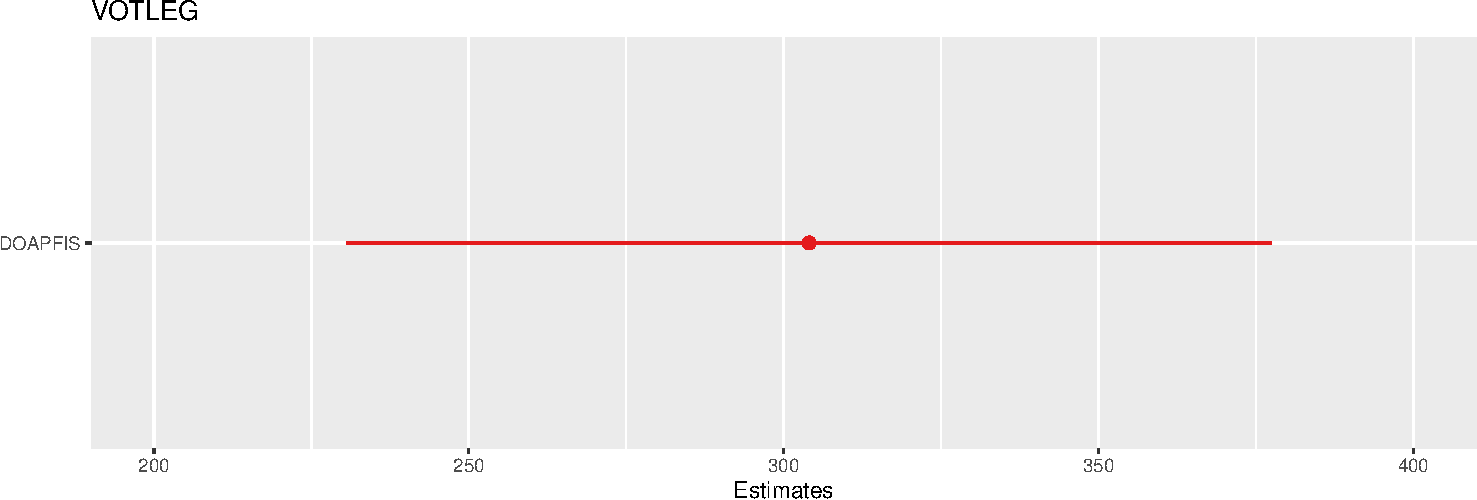
\includegraphics{aula_12_files/figure-beamer/unnamed-chunk-16-1.pdf}
\end{frame}

\begin{frame}[fragile]{Diagnósticos}
\protect\hypertarget{diagnuxf3sticos}{}
\begin{Shaded}
\begin{Highlighting}[]
\NormalTok{GGally}\OperatorTok{::}\KeywordTok{ggnostic}\NormalTok{(meu\_modelo)}
\end{Highlighting}
\end{Shaded}

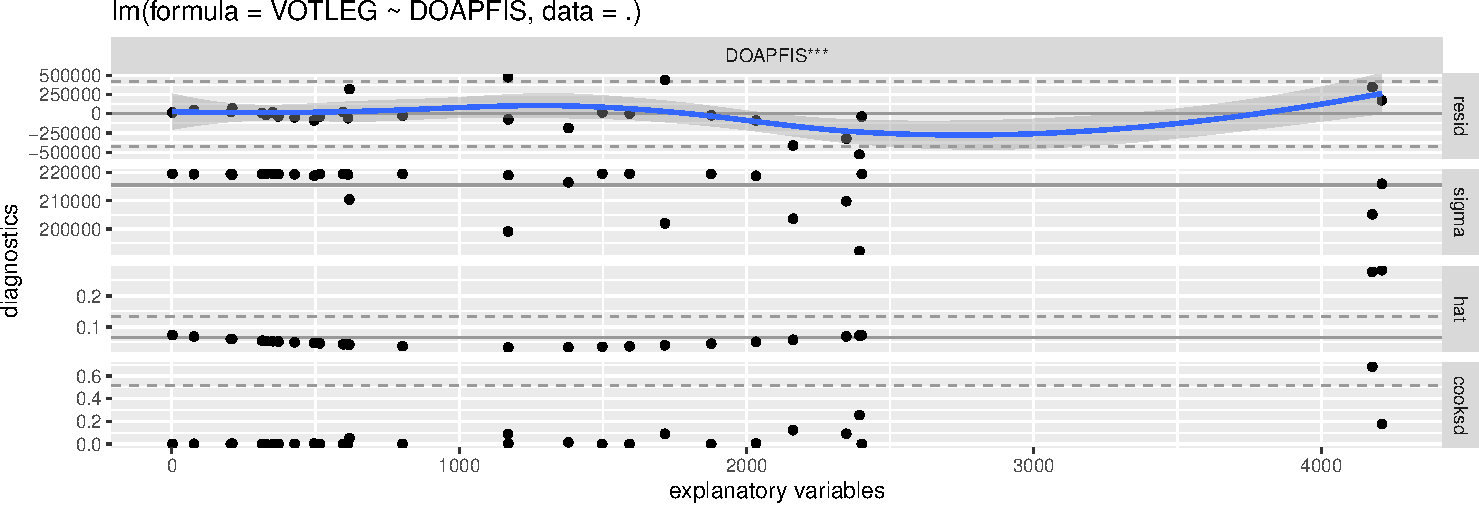
\includegraphics{aula_12_files/figure-beamer/unnamed-chunk-17-1.pdf}
\end{frame}

\begin{frame}[fragile]{}
\protect\hypertarget{section-4}{}
\begin{Shaded}
\begin{Highlighting}[]
\KeywordTok{get\_regression\_points}\NormalTok{(meu\_modelo) }\OperatorTok{\%\textgreater{}\%}\StringTok{ }\KeywordTok{mutate}\NormalTok{(}\DataTypeTok{residual=}\KeywordTok{scale}\NormalTok{(residual)) }\OperatorTok{\%\textgreater{}\%}
\StringTok{  }\KeywordTok{ggplot}\NormalTok{(}\KeywordTok{aes}\NormalTok{(}\DataTypeTok{x =}\NormalTok{ residual)) }\OperatorTok{+}
\StringTok{  }\KeywordTok{geom\_histogram}\NormalTok{(}\DataTypeTok{binwidth =} \FloatTok{.25}\NormalTok{,}\DataTypeTok{color =} \StringTok{"white"}\NormalTok{) }\OperatorTok{+}
\StringTok{  }\KeywordTok{labs}\NormalTok{(}\DataTypeTok{x =} \StringTok{"Residuos"}\NormalTok{)}
\end{Highlighting}
\end{Shaded}

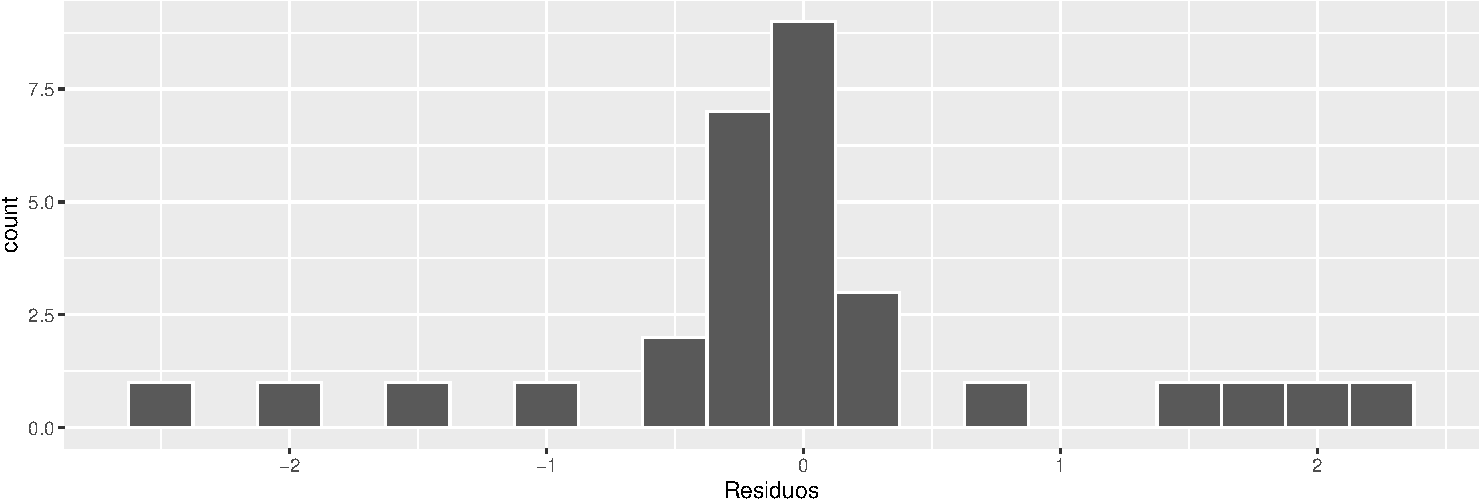
\includegraphics{aula_12_files/figure-beamer/unnamed-chunk-18-1.pdf}
\end{frame}

\begin{frame}[fragile]{}
\protect\hypertarget{section-5}{}
\begin{Shaded}
\begin{Highlighting}[]
\KeywordTok{get\_regression\_points}\NormalTok{(meu\_modelo) }\OperatorTok{\%\textgreater{}\%}\StringTok{ }\KeywordTok{mutate}\NormalTok{(}\DataTypeTok{residual=}\KeywordTok{scale}\NormalTok{(residual)) }\OperatorTok{\%\textgreater{}\%}
\StringTok{  }\KeywordTok{ggplot}\NormalTok{(}\KeywordTok{aes}\NormalTok{(}\DataTypeTok{x =}\NormalTok{ DOAPFIS, }\DataTypeTok{y =}\NormalTok{ residual)) }\OperatorTok{+}
\StringTok{  }\KeywordTok{geom\_point}\NormalTok{() }\OperatorTok{+}\StringTok{ }\KeywordTok{labs}\NormalTok{(}\DataTypeTok{x =} \StringTok{"Doações"}\NormalTok{, }\DataTypeTok{y =} \StringTok{"Residuos"}\NormalTok{) }\OperatorTok{+}
\StringTok{  }\KeywordTok{geom\_hline}\NormalTok{(}\DataTypeTok{yintercept =} \DecValTok{0}\NormalTok{, }\DataTypeTok{col =} \StringTok{"blue"}\NormalTok{, }\DataTypeTok{size =} \DecValTok{1}\NormalTok{)}
\end{Highlighting}
\end{Shaded}

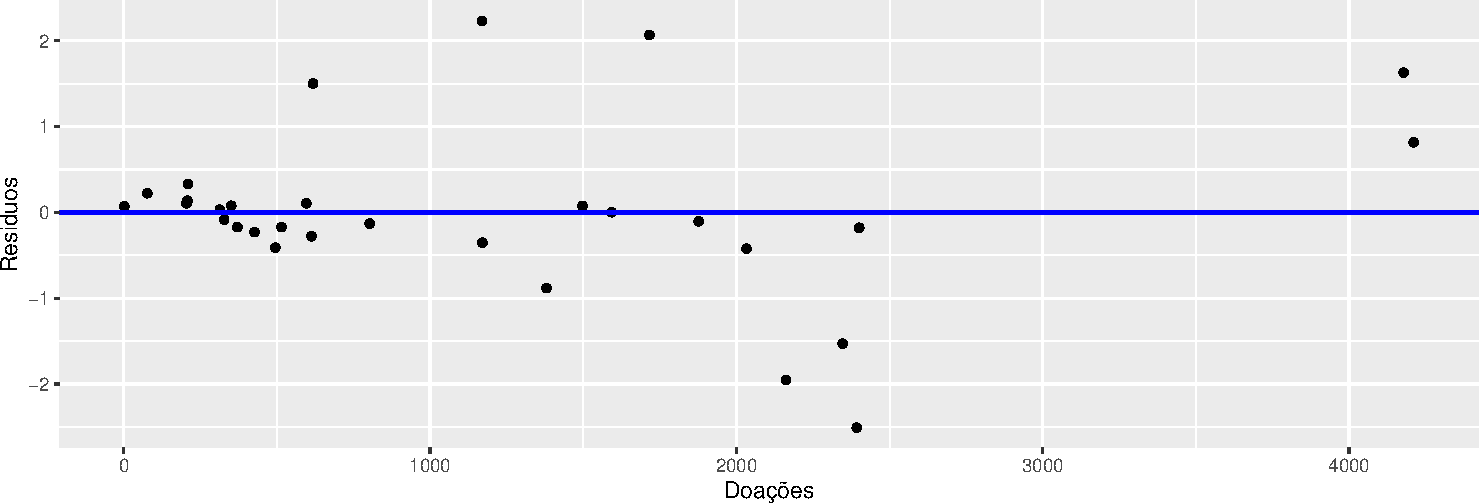
\includegraphics{aula_12_files/figure-beamer/unnamed-chunk-19-1.pdf}
\end{frame}

\begin{frame}[fragile]{}
\protect\hypertarget{section-6}{}
\begin{Shaded}
\begin{Highlighting}[]
\KeywordTok{plot}\NormalTok{(meu\_modelo,}\DecValTok{1}\NormalTok{)}
\end{Highlighting}
\end{Shaded}

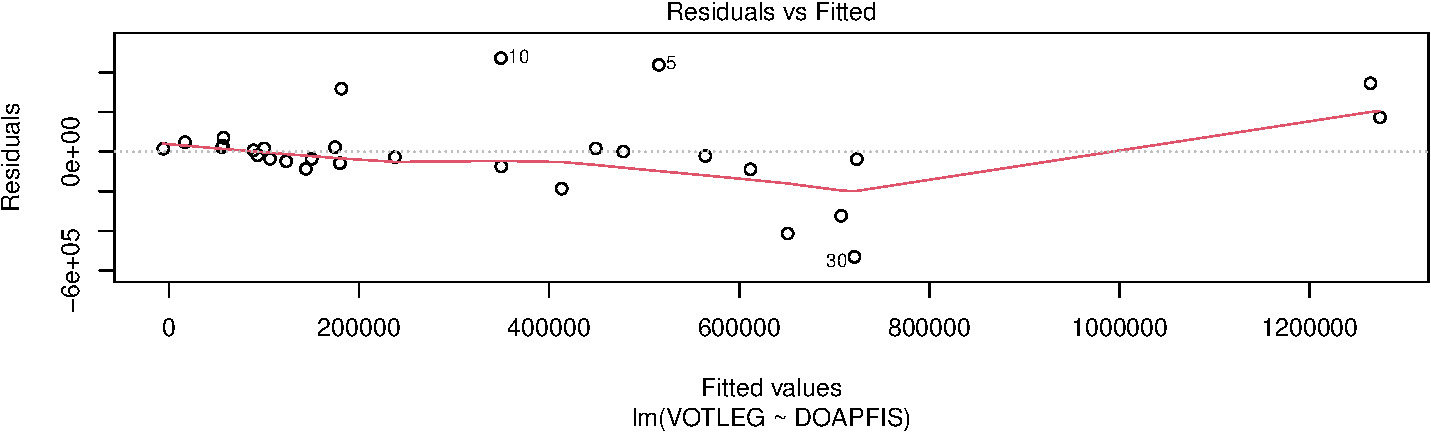
\includegraphics{aula_12_files/figure-beamer/unnamed-chunk-20-1.pdf}
\end{frame}

\begin{frame}[fragile]{}
\protect\hypertarget{section-7}{}
\begin{Shaded}
\begin{Highlighting}[]
\KeywordTok{plot}\NormalTok{(meu\_modelo,}\DecValTok{2}\NormalTok{)}
\end{Highlighting}
\end{Shaded}

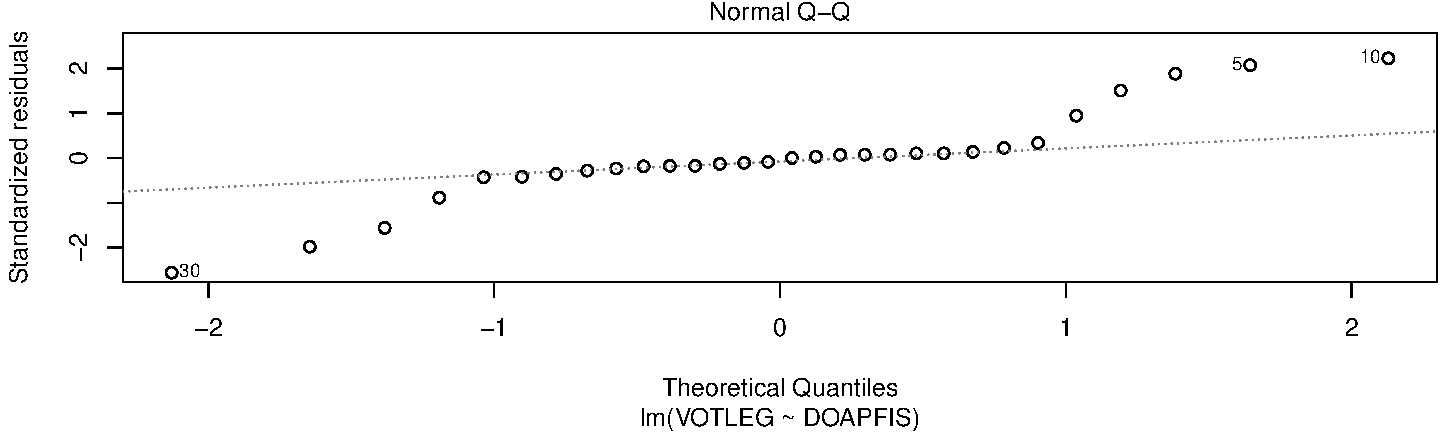
\includegraphics{aula_12_files/figure-beamer/unnamed-chunk-21-1.pdf}
\end{frame}

\begin{frame}[fragile]{}
\protect\hypertarget{section-8}{}
\begin{Shaded}
\begin{Highlighting}[]
\KeywordTok{plot}\NormalTok{(meu\_modelo,}\DecValTok{3}\NormalTok{)}
\end{Highlighting}
\end{Shaded}

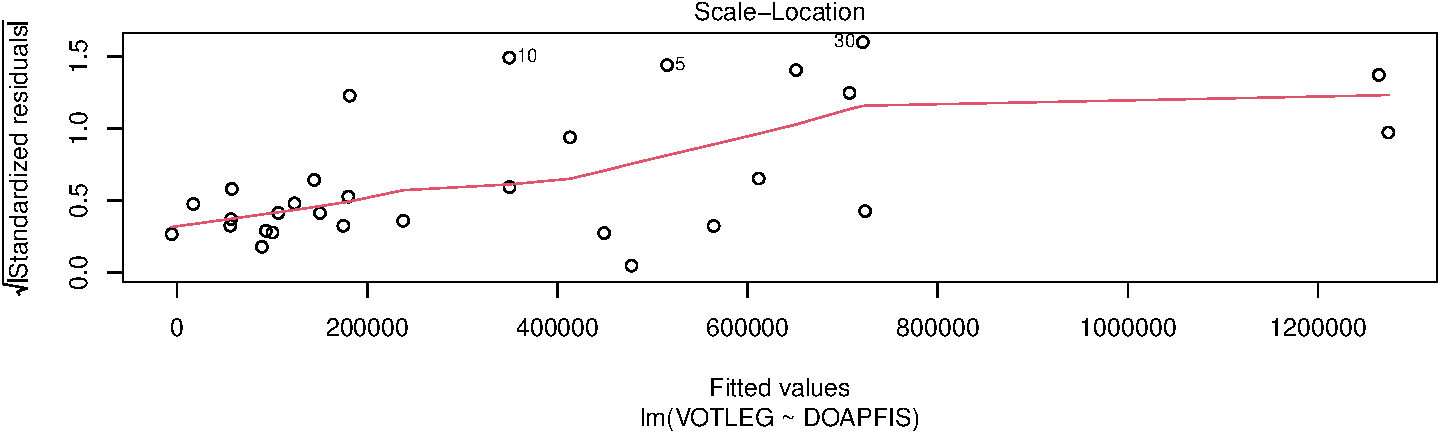
\includegraphics{aula_12_files/figure-beamer/unnamed-chunk-22-1.pdf}
\end{frame}

\begin{frame}[fragile]{}
\protect\hypertarget{section-9}{}
\begin{Shaded}
\begin{Highlighting}[]
\KeywordTok{plot}\NormalTok{(meu\_modelo,}\DecValTok{4}\NormalTok{)}
\end{Highlighting}
\end{Shaded}

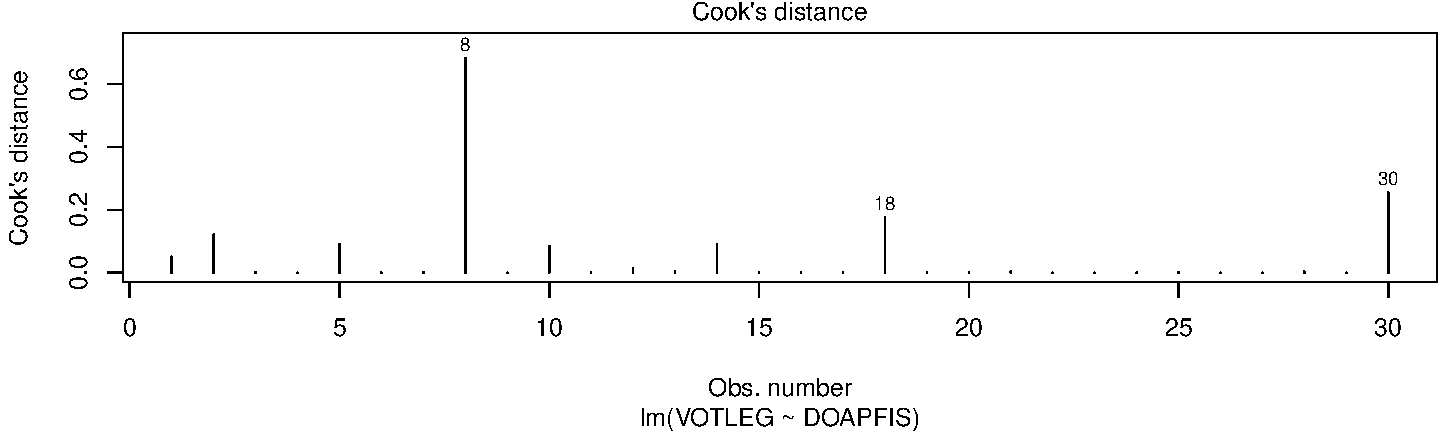
\includegraphics{aula_12_files/figure-beamer/unnamed-chunk-23-1.pdf}
\end{frame}

\hypertarget{modelos-lineares-multivariados}{%
\section{Modelos Lineares
Multivariados}\label{modelos-lineares-multivariados}}

\begin{frame}[fragile]{Modelo linear com dois preditores}
\protect\hypertarget{modelo-linear-com-dois-preditores}{}
\begin{Shaded}
\begin{Highlighting}[]
\NormalTok{(meu\_modelo2 \textless{}{-}}\StringTok{ }\NormalTok{legenda }\OperatorTok{\%\textgreater{}\%}\StringTok{ }\KeywordTok{lm}\NormalTok{(VOTLEG }\OperatorTok{\textasciitilde{}}\StringTok{ }\NormalTok{DOAPFIS }\OperatorTok{+}\StringTok{ }\NormalTok{NUMCAND, }\DataTypeTok{data =}\NormalTok{ .))}
\end{Highlighting}
\end{Shaded}

\begin{verbatim}
Call:
lm(formula = VOTLEG ~ DOAPFIS + NUMCAND, data = .)

Coefficients:
(Intercept)      DOAPFIS      NUMCAND  
  -148413.4        224.1       1685.9  
\end{verbatim}
\end{frame}

\begin{frame}[fragile]{Obtendo resultados simplificados com
\texttt{arm}}
\protect\hypertarget{obtendo-resultados-simplificados-com-arm}{}
\begin{Shaded}
\begin{Highlighting}[]
\KeywordTok{display}\NormalTok{(meu\_modelo2)}
\end{Highlighting}
\end{Shaded}

\begin{verbatim}
lm(formula = VOTLEG ~ DOAPFIS + NUMCAND, data = .)
            coef.est   coef.se   
(Intercept) -148413.43   79529.76
DOAPFIS         224.12      46.64
NUMCAND        1685.94     693.11
---
n = 30, k = 3
residual sd = 198855.86, R-Squared = 0.77
\end{verbatim}
\end{frame}

\begin{frame}[fragile]{Interpretando resultados com gráficos}
\protect\hypertarget{interpretando-resultados-com-gruxe1ficos}{}
\begin{Shaded}
\begin{Highlighting}[]
\KeywordTok{coefplot}\NormalTok{(meu\_modelo2)}
\end{Highlighting}
\end{Shaded}

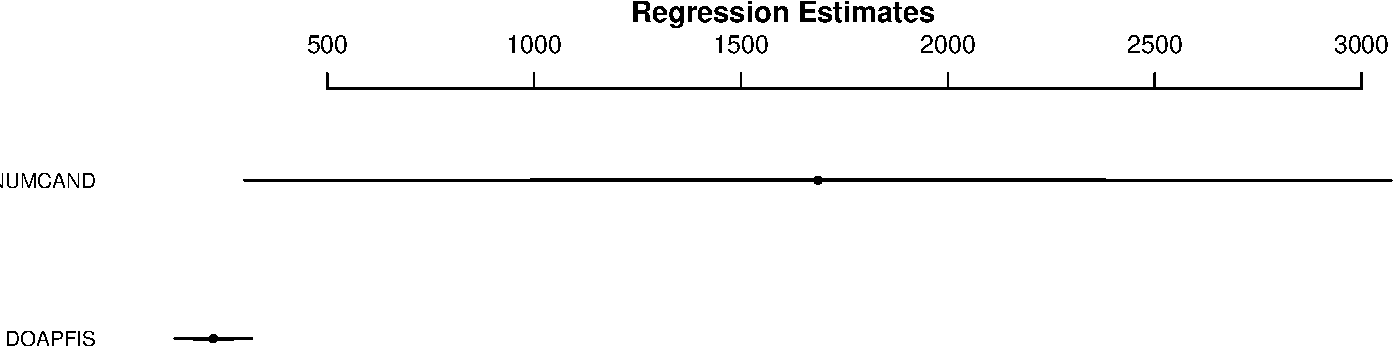
\includegraphics{aula_12_files/figure-beamer/unnamed-chunk-26-1.pdf}
\end{frame}

\begin{frame}[fragile]{Interpretando resultados com gráficos}
\protect\hypertarget{interpretando-resultados-com-gruxe1ficos-1}{}
\begin{Shaded}
\begin{Highlighting}[]
\NormalTok{sjPlot}\OperatorTok{::}\KeywordTok{plot\_model}\NormalTok{(meu\_modelo2)}
\end{Highlighting}
\end{Shaded}

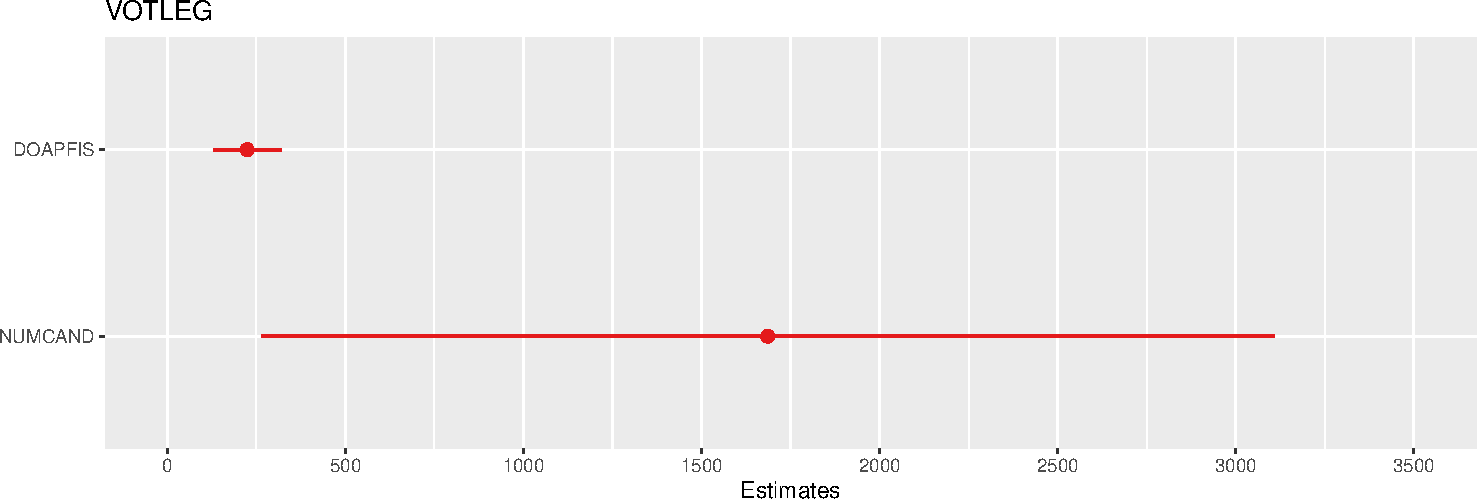
\includegraphics{aula_12_files/figure-beamer/unnamed-chunk-27-1.pdf}
\end{frame}

\begin{frame}[fragile]{}
\protect\hypertarget{section-10}{}
\begin{Shaded}
\begin{Highlighting}[]
\NormalTok{sjPlot}\OperatorTok{::}\KeywordTok{plot\_residuals}\NormalTok{(meu\_modelo2)}
\end{Highlighting}
\end{Shaded}

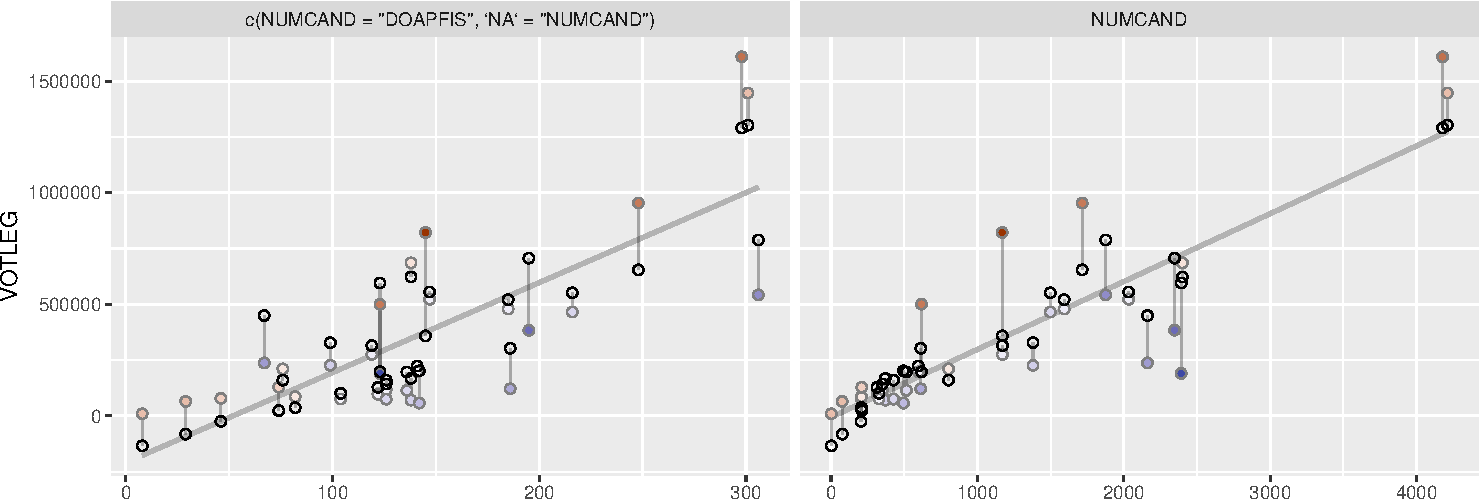
\includegraphics{aula_12_files/figure-beamer/unnamed-chunk-28-1.pdf}
\end{frame}

\end{document}
